\documentclass[a4paper,10pt]{scrartcl}
\usepackage[utf8]{inputenc}
\usepackage[english]{babel}
\usepackage{fontenc}
\usepackage{graphicx}
\usepackage{amsfonts}
\usepackage{hyperref}
\usepackage{amssymb}
\usepackage{fullpage}
\usepackage{float}
\usepackage{amsthm}
\usepackage{amsmath}
\usepackage{amssymb}
\usepackage{subcaption}
\usepackage{mathrsfs}

\title{Rapport du projet "Stratified System F"}
\subtitle{Cours 2.7.2 - Proof assistants}
\author{Adrien HUSSON - Matthieu JOURNAULT - Lucas RANDAZZO}
\date{08/03/2015}
\newcommand{\eqname}[1]{\tag*{#1}}

    \begin{document}
     \maketitle
     \section{Usage}
     Le \texttt{.tar.gz} contient un Makefile qui permet de compiler le projet en appellant \texttt{make} ou qui appellé avec la commander \texttt{make html} génère dans le sous-dossiers \texttt{/html} une documentation basée sur les commentaires du code. Ces derniers permettent généralement d'obtenir plus de détail sur le code que ce qui est décrit dans le présent rapport.
     \section{Hierarchie du Projet}
     Dans le \texttt{.tar.gz} du projet on pourra trouver les fichiers : \texttt{env\_subst.v, inference.v, init.v, lemmas\_narrowing.v, lemmas\_regularity.v, narrowing.v, red.v, regularity.v, shift\_lemmas.v}. 
%      env\_subst.v, inference.v, 
     \begin{itemize}
      \item \texttt{init.v} contient les définitions de base du projet tels que : \texttt{typ}, \texttt{term}, \texttt{env}. Il contient aussi les fonctions de base nécessaires à la manipulation des terms et des types, telles que \texttt{tshift}, \texttt{tsubst}, \texttt{get\_kind}. Enfin on peut y trouver les lemmes de base décrivant les propriétés des définitions et des fonctions précédantes. Pour un détail des intrications des lemmes, se référer à ~\ref{fig:graph}.
      \item \texttt{shift\_lemmas.v} contient les lemmes décrivant les propriétés des \texttt{shift}, la plupart découlant du lemme le plus fort : \texttt{tshift\_commut}, dont la sémantique est décrit dans la partie 2 de ce rapport.
      \item \texttt{lemmas\_regularity.v} contient les lemmes qui permettent d'établir les deux sous-lemmes \texttt{subst\_preserves\_typing} et \texttt{tsubst\_preserves\_kinding} qui sont conseillés dans l'énoncé afin de prouver \texttt{regularity}.
      \item \texttt{regularity.v} contient l'énoncé et la preuve de \texttt{regularity}, utilisant les lemmes prouvés dans \texttt{lemmas\_regularity.v}. Il est à noté toutefois que la preuve n'utilise pas \texttt{subst\_preserves\_typing} mais des lemmes qui ont permis d'établir ce résultat sont toutefois utilisés.
      \item \texttt{lemmas\_narrowing.v} contient les lemmes nécessaires pour prouver \texttt{narrowing}.
      \item \texttt{narrowing.v} contient l'énoncé et la preuve de \texttt{narrow}.
      \item \texttt{env\_subst.v}
      \item \texttt{red.v} contient la définition d'une étape de réduction par congruence, la définition de la clôture réflexive et transitive de la réduction, la définition de la forme normale et neutre d'un terme. Enfin on y trouvera les énoncés et preuves de la congruence de la réduction, de la cloture par substitution des formes normales et neutres et enfin de l'équivalence entre les termes dont la réduction termine et les termes en forme normale.
      \item \texttt{inference.v} contient les fonctions inférants les types et les kinds, d'un terme ou d'un type, ainsi que les preuves de complétude et de correction pour chacune de ces fonctions.
     \end{itemize}

      \begin{figure}
      
      \noindent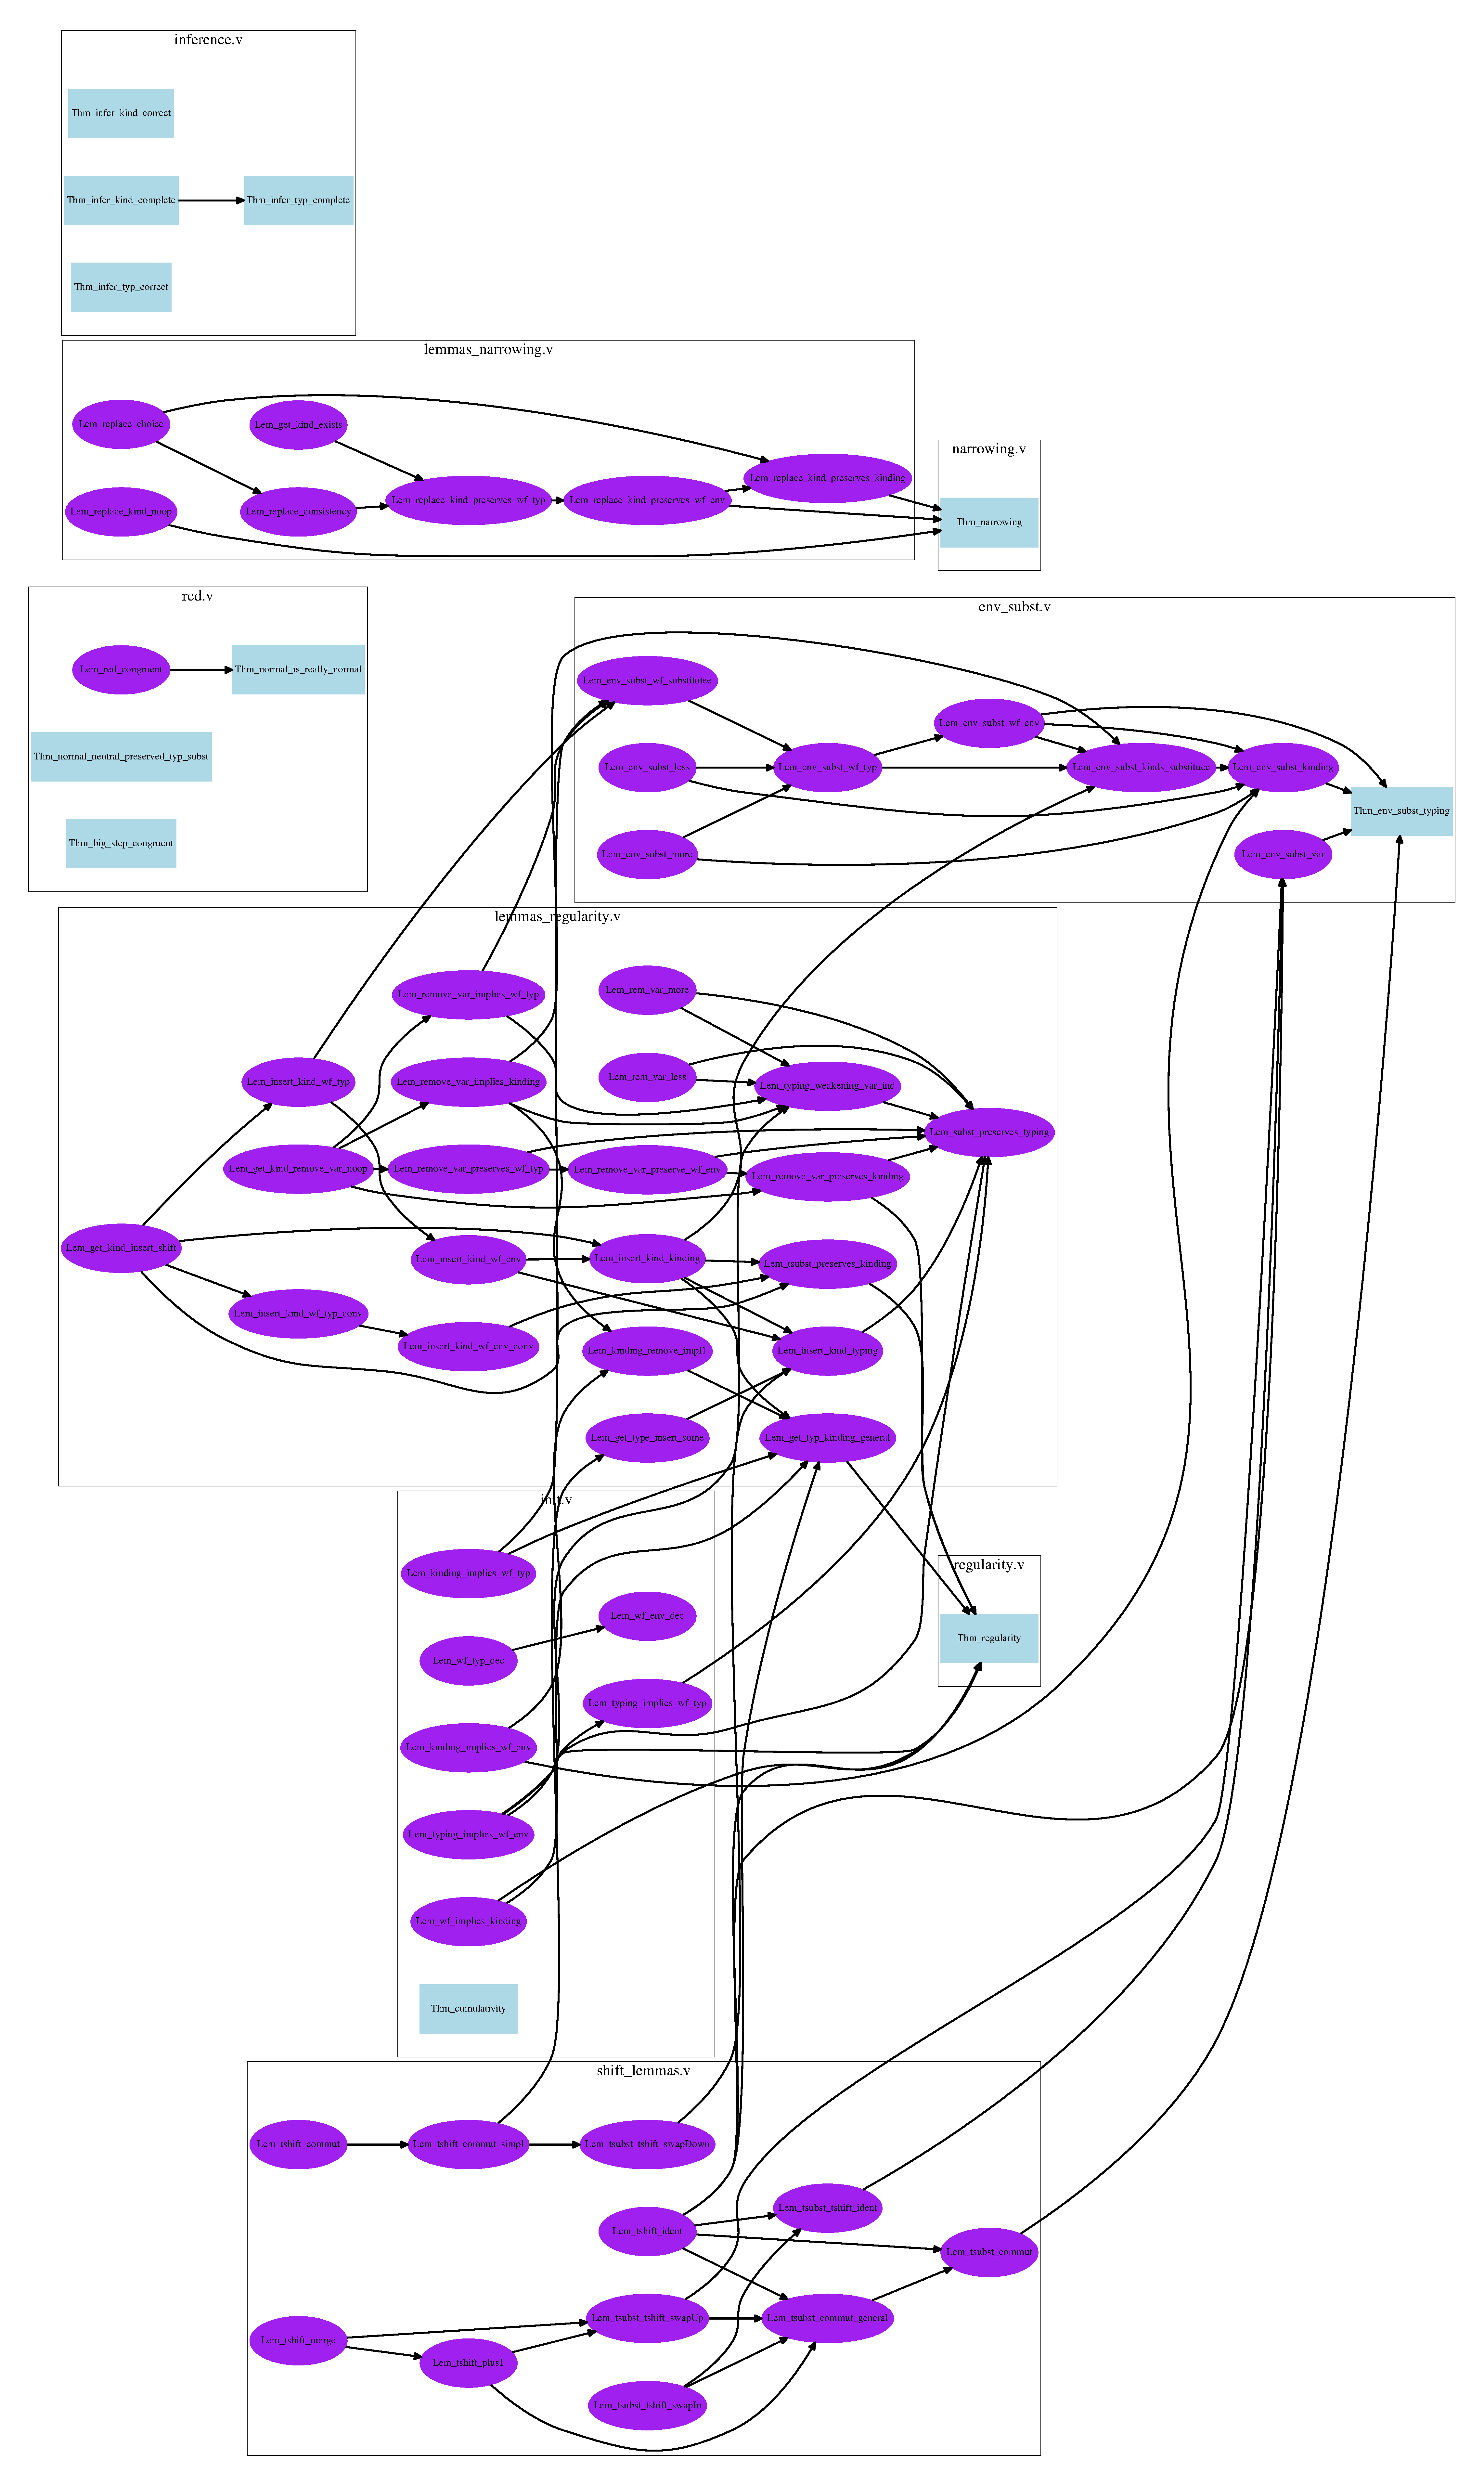
\includegraphics[width=0.9\linewidth]{../lol.pdf}
      \caption{Intrication des Lemmes et Théorèmes}
      \label{fig:graph}
      \end{figure}
      
     \section{Choix d'implémentation}
     Cette partie contient majoritairement une description des choix qui ont été fait dans \texttt{init.v}. 
     \paragraph{} Comme indiqué en commentaire dans \texttt{init.v}, on utilise les indices de Bruijn localement et globalement. On n'a pas à s'occuper d'alpha-conversion, mais beaucoup de lemmes sont dûs au shifts lors de passage sous des binders. Les environnements des variables de type et de terme sont implémenté sous la forme d'une liste commune de type \texttt{list envElem} où \texttt{envElem} est soit contient un \texttt{Typ} ou un \texttt{kind}. Ces choix rendent nécéssaire l'écriture de 3 fonctions de shifts et de 3 fonctions de substitutions que l'on peut trouver dans \texttt{init.v}. Il faut noter que l'implémentation de \texttt{subst} et de \texttt{tsubst} est fait de sorte que l'on puisse shifter toutes les variables plus grande qu'un plancher $p$ d'une valeur $n$ dans un terme $t$, appeller \texttt{shift t n p} dans le code et noter $\uparrow_p^nt$. Cette implémentation nous oblige aussi à prouver des lemmes importants pour de nombreuses parties du code et que l'on peut trouver dans \texttt{shift\_lemmas.v}. On résume ici l'énoncé de ces lemmes qui sont nécessaires à la preuve de nombreux lemmes de notre projet : 
     \begin{align} 
      \forall t,\ p,\ \Big\uparrow_p^0 t &= t \eqname{\texttt{(tshift\_ident)}} \\
      \forall t,\ a,\ c,\ d,\ p,\ \Big\uparrow_{p+d}^c \Big\uparrow_p^a t &= \Big\uparrow_{p}^a \Big\uparrow_{(d-a+p)}^c t \eqname{\texttt{(tshift\_commut)}} \\
      \forall t,\ c,\ d,\ \Big\uparrow_{d+1}^c \Big\uparrow_0^1 t &= \Big\uparrow_{0}^1 \Big\uparrow_{c}^d t \eqname{\texttt{(tshift\_commut\_simpl)}} \\
      \forall T,\ U,\ X,\ n,\ n \leq X \Rightarrow \Big\uparrow_{X}^1 (T[n\rightarrow U]) &= (\Big\uparrow_{(X+1)}^1T)[n \rightarrow \Big\uparrow_X^1U] \eqname{\texttt{(tsubst\_tshift\_swapN)}}
      \end{align}
      \paragraph{} Il est important de noter que le choix d'avoir une fonction de shift qui shift toutes les valeurs d'une certaines quantité plutôt que d'appeller plusieurs fois une fonction qui effectue un seul shift sur chaque variable nous a permis de prouver les lemmes précédants assez rapidemment en se ramenant à des équations sur les entiers pour chaque variable.
     
     \section{Automation tools}
         Nous avons utilisé les techniques simples d'automatisation suivantes :
     \begin{itemize}
     \item Ajout de lemmes d'arithmétique simple à {\tt auto}.
     \item Ajout des constructeurs de nos types inductifs à {\tt auto}.
     \item La tactique {\tt inv} qui substitue les égalités générées par {\tt inversion}.
     \item {\tt auto} résoud les contextes trivialement absurdes.
     \item Ajout de lemmes/théorèmes utiles à {\tt auto}, par exemple {\tt cumulativity}.
     \end{itemize}
     \paragraph{}Certaines sections ont particulièrement profité de l'automatisation, par exemple {\tt inference.v} qui
     descend récursivement dans le corps des fonctions d'inférence, ce qui permet de prouver la plupart des
     lemmes de correction/complétude de l'inférence avec {\tt eauto}. {\tt shift\_lemma.v} contient aussi
     une tactique {\tt destruct\_match} qui permet de faire automatiquement de la disjonction de cas
     sur l'ordre des entiers utilisés dans {\tt tshift / tsubst }.

     \section{TONAME}
     Cette partie du rapport reprend certains fichiers en revenant cette fois sur les difficultés que nous avons rencontré dans chacune des parties et en essayant de mettre en avant ce qui aurait pû être amélioré, à la fois dans le code et dans la manière avec laquelle nous avons essayé de répondre au problème. D'une manière générale nous avons commencé à travailler en parrallèle sur les différentes parties du code, en partant des définitions de \texttt{init.v} et en essayé de répondre à des questions qui nous semblaient distinctes. Toutefois ils nous a fallu revenir plusieurs fois sur les choix à la fois d'implémentation que nous avions fait au début mais aussi sur des définitions qui étaient fausses.
     \begin{itemize}
      \item \texttt{init.v} Nous avons pris les définitions prises par l'énoncé, nous avons donc rapidemment pu coder les définitions et les prédicats inductifs de cette partie ainsi que les lemmes associés.
      \item \texttt{shiftlemma.v} Les lemmes qui se trouvent dans ce fichier, bien que facile et rapide à démontrer ont été difficile à trouver (parce qu'il était nécessaire d'essayer de commencer à essayer de faire les preuves de lemmes plus importants pour voir de quels résultats nous avions besoin, mais aussi parce que nous avons essayé de synthétiser tous les lemmes dont nous aurions besoin par la suite et portant sur cette partie en un minimum de lemme).
      \item \texttt{red.v} Cette partie du projet, assez indépendante des autres est une de celle qui nous a pris le moins de temps. En effet il n'était pas nécessaire d'établir des lemmes intermédiaire et les résultats découlaient assez rapidemment des définitions. On peut noter que cette partie contient une preuve que les termes en forme normal sont bien ceux dont la réduction termine et réciproquement.
     \end{itemize}
     

    \end{document}
